\section {Evaluation}
\label{sec:eval}
In this section, we describe our evaluation experiments and results.

\subsection{Dataset Statistics and Evaluation}
\label{subsec:human baseline}

The current version of the dataset~\footnote{We have processed $941$ scripts and 
manually labeled $300$ of them with relationships at present.
 A full dataset (with much larger expected scale) will be made 
public once ready. The current version can be downloaded at: 
\url{http://adapt.seiee.sjtu.edu.cn/~kzhu/dialogue_relationship_dataset.rar}.}
%For readers who want to have a copy of the current dataset,	please contact the first arthor.} is described in Table \ref{table:dataset}. 
contains $6,307$ labelled sessions of dyadic dialogues, 
which take place between $700$ pairs of characters across $300$ movies. 
The average number of turns in each dialogue is $8.44$, 
while it varies greatly (standard deviation is $6.43$). 
Of the $3,114$ sessions that fall into the category of family or 
workplace relationships, $1,829$ of them belong to the larger (workplace) class. 
So our majority baseline is $58.7\%$. We split the dataset into $2,770$ train samples and $344$ test samples. Both human and algorithm performance are later measured on this test set to ensure fair comparison. 
\begin{table}[h!]
	\centering
	\small
	\begin{tabular}{@{}lrr@{}}
		\toprule
		\textbf{}                & 13 classes & family/workplace \\ \midrule
		\# Pair of Speakers      & 693        & 157/243             \\
		\# Sessions              & 6,307       & 1,285/1,829        \\
		\# Turns                 & 53,210     & 10,382/13,909           \\
		Sessions per pair (min)  & 1          & 1                \\
		Sessions per pair (mean) & 9.10       & 7.79             \\
		Sessions per pair (max)  & 71         & 71               \\
		Turns per session (min)  & 3          & 3                \\
		Turns per session (mean) & 8.44       & 7.8              \\
		Turns per session (max)  & 155        & 155              \\\midrule
		Inter-labeler Agreement & 82.3\%     & 96.6\%           \\ \bottomrule
	\end{tabular}
	\caption{Statistics about the obtained dataset.}\label{table:dataset}
\end{table}

The following two experiments verify the accuracy of obtained 
labels and validity of this proposed task.

\subsubsection*{Second-Annotator Verification}
Due to excessive cost of the annotation task, 
we are not able to commit multiple annotators on the labelling task. 
But to compensate that, we verify the accuracy of annotation by 
having a second person label 100 pairs with the same experimental settings. 
The inter-annotator agreement (kappa) is $82.3\%$ for 13-classes and $96.6\%$ for 
the binary classification. 
This indicates that incorrect labels are limited to a small number, and the annotation by the first human is 
reliable.
%wrong labels account for a very small, 
%acceptable proportion of the whole dataset.


\subsubsection*{Human Baseline}
We pose the 13-class relationship inference task to human volunteers in a preliminary survey and the average accuracy is only $39\%$. This means for most dialogue segments we extracted, there is not enough information even for humans to determine between the fine-grained 13 classes. 
Therefore, we focus on the simpler family/workplace binary 
classification problem in this paper. 
Four volunteers, each having at least 4 year's experience in English-speaking 
country, participated in our human performance test. 
Provided with dialogue transcripts (the speakers 
names are presented by `A' or `B') only, the volunteers were asked to 
enter their best guess about the two speakers relationship along with 
a confidence score(0-4, 0 means random guess and 4 means almost certain). 
Their answers covered all dialogues in test set, 
with each sample assessed by 2 participants.

The average accuracy is $81.69\%$ and  
inter-participant agreement (kappa) is $77.5\%$. 
The mean of reported confidence score is $2.76$. 
These results 
\begin{enumerate}[label=(\roman*)]
	\item verify human's ability on this task: they can get the right choice in more than $80\%$ cases with moderate confidence;
	\item show that this task is non-trivial: 
	only $40.5\%$ answers report a high confidence score of 3 or 4, 
	which means in most samples no obvious evidence exists,
	and even people have to look for subtle hints and do some guesswork.
	\item from another aspect verify the accuracy of annotation.
\end{enumerate}

\subsection{Classification Experiments}   
With all the features in \secref{sec:method} extracted, we use Logistic Regression as the 
classifier to measure the indicative power of different features and their combinations. 

Binary classification accuracy of baseline methods and our approaches are shown in \tabref{Tab:result}. 
Logistic Regression with Bag-of-differential-Words, Address terms and linguistic pattern features 
achieves highest computational accuracy of $78.49\%$ and a Matthews Correlation Coefficient (MCC) of $0.554$.
This is significantly higher than competitive neural network approaches and is very close to the $81.69\%$ human baseline. 
                                                                  
\begin{table}[th]
	\centering
	\small
	\begin{tabular}{@{}lcc@{}}
		\toprule
		\textbf{Approach}                         & \textbf{\begin{tabular}[c]{@{}l@{}}Accuracy on \\ test set\end{tabular}} & \textbf{\begin{tabular}[c]{@{}l@{}}Accuracy on \\ 8-fold cross \\validation\end{tabular}} \\ \midrule
		Majority Baseline                 & 58.35\%                    & /                               \\
		CNN                                 & 68.60\%                    &     /                                                                           \\
		LSTM                                 & 66.57\%                     & /                                                                               \\
		3-level hierarchical \\attentional LSTM & 70.35\%                     & /                                                                               \\
			Human Baseline                    & \textbf{81.69\%}             & /                                   \\ \midrule
		{[}LIWC{]}+LR                     & 67.44\%              & 67.37\%                             \\
		{[}BOW{]}+LR                      & 72.09\%              & 71.67\%                             \\
		{[}d-BOW{]}+LR & 76.22\%               & 74.89\%                            \\	
		{[}d-BOW+LIWC{]}+LR            & 76.45\%              & 73.86\%                             \\	
		{[}d-BOW+Addr{]}+LR   & 78.19\%              & \textbf{75.34\%}                             \\
		\textbf{{[}d-BOW+Addr+LP{]}+LR}   & \textbf{78.49}\%              & 75.05\%                             \\ \bottomrule
	\end{tabular}
	\caption{Comparisons of baseline methods and our feature-engineering approach.}\label{Tab:result}
\end{table}

\subsubsection*{Indicative Features}
\begin{figure*}[th!]
	\centering
	\begin{tabular}{@{}cccc@{}}
		\includegraphics[width=.464\textwidth]{d-bow.eps} &
		\includegraphics[width=.24\textwidth]{liwc.eps} &
		\includegraphics[width=.248\textwidth]{lp.eps} 
	\end{tabular}
	\caption{Mean and standard error of features with large disparity
		across the two classes. The y-axis stands for average score on each feature.} \label{fig:compare}
\end{figure*}
In this part we analyze which features are important in our model by examining the coefficients 
and p-values in logistic regression for each feature we applied. 

The most informative features are d-BOW vectors. Our $400$-bit d-BOW vector achieves $4\%$ higher accuracy than $7112$-bit traditional BOW vector.
Address terms are also very useful,  
but their advantage is limited because $80\%$ of our samples contain 
no address term at all. No significant difference between one-hot encoding and average word vector representation is found in experiments.
LIWC actually performs well alone($67.44\%$). However, 
as another lexical-level feature, it rarely brings extra information 
when combined with d-BOW vectors. Results are similar 
if we look into the p-values of each single feature (one bit in 
the feature vector, for example, count of a certain word in d-BOW). 
Features with smallest p-values are listed in \tabref{Tab:indicative features}. Not surprisingly, it shows some overlapping with words with most imbalanced distributions (see \tabref{table:dbow}).

\begin{table}[t]
	\small
	\centering
	\begin{tabular}{|l|l|l|}
		\hline
		\multirow{2}{*}{+} & Ngrams  & \begin{tabular}[c]{@{}l@{}}`needed', `know think', `go out',\\ `the kids', `cook', `house',\\ `school', `closet'\end{tabular} \\ \cline{2-3} 
		& Address & `daddy', `dear', `dad', `lord'                                                                                                \\ \hline
		\multirow{2}{*}{-} & Ngrams  & \begin{tabular}[c]{@{}l@{}}`it in', `use', `little', `does',\\ `know it', `the', `job', `fuck'\end{tabular}                   \\ \cline{2-3} 
		& Address & `sir', `mr', `captain'                                                                                                        \\ \hline
	\end{tabular}
	\caption{Single features with p-values $\le 0.02$. Here ``+'' stands for positive coefficients(family) and ``-'' negative(workplace). No syntactic feature occurs even if we set the threshold to $p=0.05$.}
	\label{Tab:indicative features}
\end{table}

Feature's indicative power corresponds to the imbalance of their distribution,
as shown in \figref{fig:compare}. We can see that some tokens and bigrams significantly occur more in one relationship than another, 
and so as some LIWC features. 
Syntactic structures and linguistic patterns show less variance in 
their distribution, and their help in the classification 
is also limited: LR with syntactic complexity measurements and linguistic pattern (LP) features can't do better than the majority baseline. 
As shown in the bottom of \tabref{Tab:result}, LP exists in our best feature combination, but the contribution is small 
and likely incidental. 
Despite this disappointing negative result, 
we still believe those aspects of dialogues are important. 
Future work may be able to verify this by better identifying and 
describing those characteristics.
